\tikzset{
  treeInode/.style = {align=center, inner sep=0pt, text centered,
    font=\sffamily},
  treeEnode/.style = {align=center, inner sep=0pt, text centered,
    font=\sffamily},
  arn_n/.style = {treeInode, circle, black, draw=black,  
	  text width=1.5em},% arbre rouge noir, noeud noir
  arn_x/.style = {treeEnode, rectangle, draw=black,
    minimum width=1.5em, minimum height=1.5em}% arbre rouge noir, nil
}
\usetikzlibrary{patterns}
\begin{tikzpicture}[-,>=stealth',level/.style={sibling distance = 5cm/#1,
  level distance = 1cm}] 
\node[arn_n]{6}
	child{
		node[arn_n]{3}
		child{
			node[arn_n]{2}
			child{
				node[arn_n]{1}
				child{
					node[arn_x]{0.5}
				}
				child{
					node[arn_x]{1.5}
				}
			}
			child{
				node[arn_x]{2.5}
			}
		}
		child{
			node[arn_n]{5}
			child{
				node[arn_n]{4}
				child{
					node[arn_x]{3.5}
				}
				child{
					node[arn_x]{4.5}
				}
			}
			child{
				node[arn_x]{5.5}
			}
		}
	}
	child{
		node[arn_x]{6.5}
	}
; 
\end{tikzpicture}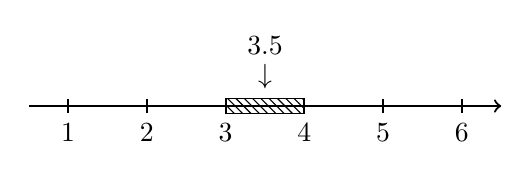
\begin{tikzpicture}[scale=5]
\draw[->, thick] (-0.1,0) -- (1.1,0);
\foreach \x/\xtext in {0/1,0.2/2,0.4/3,0.6/4,0.8/5,1.0/6}
    \draw[thick] (\x,0.5pt) -- (\x,-0.5pt) node[below] {\xtext};

\draw (0.5,3pt) node[above] {3.5};
\draw (0.5,0.5pt) node[above] {$\downarrow$};
\draw[pattern=north west lines, pattern color=black] (0.4,-.02) rectangle (0.6,0.02);
\end{tikzpicture}
